
\section{Progettazione Concettuale (Teoria)}
Quale tipo di formalismo si utilizza? Non è il caso di utilizzare il modello E/R perché è troppo potente, perché la rappresentazione di concetti semplici risulta troppo articolata.\newline
Alcuni saltano questo processo e passano direttamente allo schema logico (a stella), ma non è una mossa intelligente.\newline
Il formalismo utilizzato nel corso è ad-hoc, e si chiama DFM (Dimensional Fact Model).
Il livello concettuale è molto utile anche per la documentazione.
\subsection{DFM}
Il DFM è un modello concettuale grafico ad-hoc. La rappresentazione generata dal DFM consiste in un insieme di \textbf{schemi di fatto}. Gli elemtni modellati sono infatti i fatti, le misure, le dimensioni e le gerarchie. Il DFM fornisce anche una documentazione espressiva e non ambigua.\newline
I fatti, le dimensioni e le misure sono rappresentate nel seguente modo nel DFM:
\begin{figure}[H]
	\begin{center}
		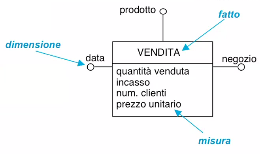
\includegraphics[width=0.5\linewidth]{img/dfm.png}
		\caption{Fatti, Dimensioni e Misure in DFM}
	\end{center}
\end{figure}
\noindent Un fatto esprime una associazione molti a molti tra le dimensioni. Nel caso riportato tra data prodotto e negozio ci sono associazioni molti a molti. Inoltre:\newline
prodotto, negozio, data $ \xrightarrow{} $ quantità venduta, incassi, num. clienti, prezzo unitario\newline
In pratica è sempre vero che date tante dimensioni $d1, d2, ..., dn$ e tante misure $m1, m2, ..., mn$ allora:
$d1, d2, ..., dn \xrightarrow{} m1, m2, ..., mn$
Questo significa che data una tripla dei valori delle dimensioni ottengo l'istanza dei valori presenti nella cella corrispondente nel cubo.\newline
\subsubsection{Gerarchie}
Una gerarchia è un albero orientato in cui i nodi sono attributi dimensionali, rappresentati come un pallino. Gli archi sono associazioni molti a uno, ovvero una dipendenza funzionale.\newline
La dimensione è la radice dell'albero.\newline
Il verso del cammino è implicito, le frecce vanno solo verso l'esterno dell'albero a partire dalla radice.
\begin{figure}[H]
	\begin{center}
		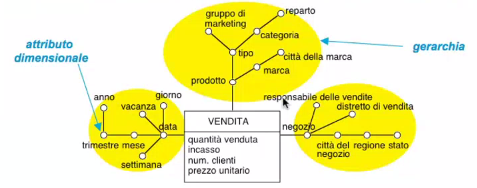
\includegraphics[width=0.5\linewidth]{img/ger.PNG}
		\caption{Esempio di gerarchie}
	\end{center}
\end{figure}
\noindent Nell'esempio un tipo è seguito da un gruppo di marketing, un reparto segue molte categorie, un prodotto appartiene ad una categoria. Un negozio ha un solo responsabile vendite.\newline In pratica se esistono due pallini collegati direttamente da un cammino orientato allora esiste una dipendenza transitiva di tipo uno a molti tra loro.\newline
Scegliamo ora due pallini che non sono collegati da un cammino orientato, per esempio categoria e marca. In questo caso il tipo di associazione è molti a molti.\newline
Parlando della data invece, la settimana non può stare tra data e mese perché alcune settimane stanno a cavallo tra due mesi.\newline
Se la cardinalità di anno è 3, quanto è la cardinalità di data? 365*3, arrotondiamo a 1000. Il dominio di mese sarà 12 * 3, e non 12, altrimenti non ci sarebbe la dipendenza funzionale tra mese ed anno, il nome è ambiguo, un nome più corretto sarebbe \textit{mese in anno}. In trimestre per lo stesso ragionamento ha cardinalità 3*4.\newline
Problema: all'utente interessa fare analisi su cosa succede durante un determinato mese indipendentemente dall'anno. Come dovremmo fare? Aggiungendo un nuovo pallino (l'effettivo mese, denotiamolo con mese') che parte da mese. Il pallino non può partire da data, perché anche se la dipendenza funzionale molti a uno è rispettata non è corretta invece la molti a molti che si crea implicitamente tra mese' e mese.\newline\newline
Un'istanza del cubo è una particolare situazione in cui si trova il cubo, si tratta di un insieme di celle che prendono il nome di \textbf{eventi primari}. Quindi un evento è una particolare occorrenza del fatto. Ad ogni evento è associato un record con le relative misure.\newline
Data una n-upla di attributi dimensionali stiamo specificando un group-by-set, ovvero un livello di aggregazione, cioè un insieme di GROUP BY. Fissato un group-by-set sto implicitamente definendo un insieme di eventi secondari. In pratica da molti cubi estremamente dettagliati passiamo a meno cubi più aggregati.\newline
Quali sono i possibili group-by-set? In riferimento all'esempio di prima, qualche esempio è:
\begin{itemize}
	\item {data, prodotto, negozio} (il più fine possibile);
	\item {mese, categoria, regione} (un attributo da ciascuna gerarchia, aggregazione possibile);
	\item {mese, categoria, negozio};
	\item {mese, categoria} (valido, è un aggregazione totale su tutti i negozi);
	\item {mese} (un cubo in cui vedo tutte le vendite mensili per tutti i negozi e tutti i prodotti. In questo caso la cardinalità degli eventi secondari è 36);
	\item {} (group-by-set vuoto, c'è un unico evento secondario);
	\item {categoria, marca} (valido anche se stanno sulla stessa gerarchia, il risultato sarà molto sparso ma il risultato è perfettamente sensato).
\end{itemize}
group-by-set non validi:
\begin{itemize}
	\item {tipo, reparto} (non valido, esiste un cammino orientato tra i due pallini, quindi la relazione tra i due è di tipo uno a molti. Non ha senso questo group by set perché tipo è un livello più fine di reparto, che quindi non verrebbe neanche calcolato nel GROUP BY);
	\item {negozio, regione} (per lo stesso motivo).
\end{itemize}
Morale: è possibile effettuare group-by-set con pallini che sono in relazione molti a molti tra loro.\newline
I possibili group-by-set sono tantissimi, il numero è esponenziale, poco meno di $2^n$.\newline

\begin{figure}[H]
	\begin{center}
		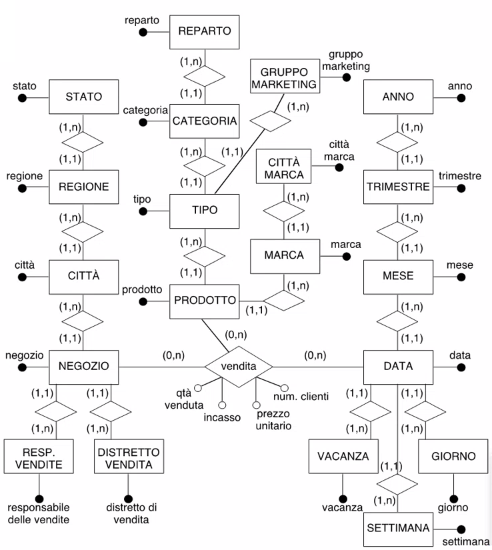
\includegraphics[width=0.7\linewidth]{img/erger.png}
		\caption{Corrispondenza con E/R}
	\end{center}
\end{figure}

\noindent Ogni evento primario entra esattamente in un evento secondario. Questo è assicurato perché ogni arco della gerarchia è di tipo molti a uno, componendoli per fare un roll-up ogni evento primario finisce in uno secondario.\newline

\subsection{Costrutti avanzati}

\subsubsection{Attributo descrittivo}
\begin{info}[Quante volte compare questo costrutto?]
	Molto spesso, è praticamente onnipresente.
\end{info}
Un attributo che contiene informazioni aggiuntive su un attributo dimensionale di una gerarchia a cui è connesso.
tra l'attributo dimensionale padre e l'attributo descrittivo figlio c'è una dipendenza funzionale. Si denota con una linea senza pallino denotata da un nome. Un attributo descrittivo è sempre una foglia e non può avere figli. La differenza da un attributo dimensionale è l'impossibilità di fare GROUP BY.\newline
Motivazioni:\newline
\begin{itemize}
	\item l'attributo descrittivo potrebbe essere legato al padre da un'associazione uno a uno. L'operazione di roll-up non porterebbe quindi a nulla.
	\item Se il dominio dell'attributo descrittivo è continuo e non discreto l'operazione di GROUP BY ha poco senso, quindi o si rendono descrittivi o si convertono in dimensionali, per esempio creando dei range (un esempio è il peso).
	\item A volte non ha senso fare aggregazione, per esempio su un attributo di tipo nome e cognome. Se nome e cognome fossero di tipo dimensionale il GROUP BY avrebbe poco senso a fini analitici, e quindi si mettono descrittivi.
\end{itemize}

\subsubsection{Archi opzionali}
\begin{info}[Quante volte compare questo costrutto?]
	Nella realtà molto spesso, a lezione e agli esami un po' più di rado.
\end{info}
Un arco opzionale può non esserci. Si denota con una piccola barra perpendicolare sull'arco. Per alcune istanze quindi abbiamo un valore dell'attributo dimensionale, per altre no. Non necessariamente gli attributi opzionali sono sempre foglie, potrebbero essere un'intera gerarchia.In questo caso si taglia su tutto l'albero che c'è a valle.

\begin{figure}[H]
	\begin{center}
		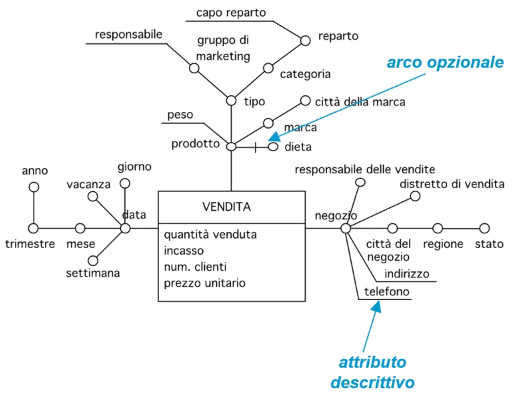
\includegraphics[width=0.7\linewidth]{img/optdesc.png}
		\caption{Costrutti: Arco opzionale, Attributo descrittivo}
	\end{center}
\end{figure}

\subsubsection{Gerarchia Condivisa}
\begin{info}[Quante volte compare questo costrutto?]
	Abbastanza spesso.
\end{info}
Remember when Rizzi said "Le gerarchie sono alberi?". Well, that was a fucking lie.\newline
Un albero è aciclico, un grafo non necessariamente. Nelle gerarchie è possibile avere cicli. Addirittura di sono quattro possibili modi per farlo, il primo modo è questo. Si tratta del ciclo più soft. Il costrutto grafico è abbastanza semplice ed orientato al riuso. In pratica è possibile riusare una gerarchia. Nell'immagine che segue per esempio (ultimo esempio) la città viene condivisa tra cliente e magazzino. La stessa cosa vale per data. Graficamente si rappresenta con un doppio pallino. La gerarchia geografica e la gerarchia temporale sono esempio classici dell'utilizzo di questo costrutto.\newline\newline
Un altro caso in cui viene utilizzato è il primo esempio dell'immagine. In questo caso la gerarchia in comune copre il dominio dei numeri di telefono. Nel caso in cui si entri dallo stesso posto (in questo caso da un fatto) più volte in una gerarchia condivisa è necessario specificare dei ruoli che danno un significato all'arco. Un altro esempio è uno studente che può avere più collegamenti con una città (di residenza e di nascita).\newline
La freccia non è obbligatoria, o meglio lo è solo in casi particolari, per essere sicuri direi di metterla sempre.\newline

\begin{figure}[H]
	\begin{center}
		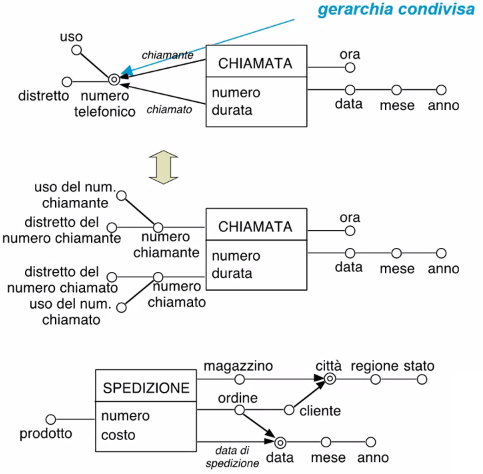
\includegraphics[width=0.7\linewidth]{img/gercond.png}
		\caption{Costrutto: Gerarchia Condivisa}
	\end{center}
\end{figure}

\subsubsection{Convergenza}
\begin{info}[Quante volte compare questo costrutto?]
	Un po' meno frequenti delle gerarchie condivise.
\end{info}
Il secondo costrutto in modo di creare un ciclo nella gerarchia. Molto simile alla gerarchia condivisa, ma più forte perché aggiunge un vincolo sulle istanze che nelle gerarchie condivise non esiste.
Una condivisione non implica niente sulle istanze, che non devono necessariamente coincidere.\newline
Nell'esempio che segue, da un negozio esce un distretto di vendita che sta in uno stato. Anche il negozio sta in una città che sta in uno stato. Se desideriamo che il distretto in cui si trova il negozio faccia parte dello stesso stato in cui il negozio si trova, allora è necessario utilizzare una convergenza.\newline
Utilizzando una gerarchia condivisa questo vincolo non esiste. Il distretto potrebbe trovarsi in Francia anche se il negozio è in Italia. La convergenza si rappresenta come la gerarchia condivisa ma non ha il pallino doppio.\newline
Non ha senso avere una convergenza tra due attributi che appartengono a dimensioni diverse.

\subsubsection{Attributo cross-dimensionale}
\begin{info}[Quante volte compare questo costrutto?]
	Raro.
\end{info}
Utilizzato per esprimere dipendenze funzionali composte. Due o più attributi ne determinano un altro congiuntamente. L'attributo può essere dimensionale o descrittivo. Per definire l'IVA non basta solo la categoria o solo lo stato, servono necessariamente entrambi, quindi:\newline
categoria, stato  $\xrightarrow[]{}$ IVA
\begin{figure}[H]
	\begin{center}
		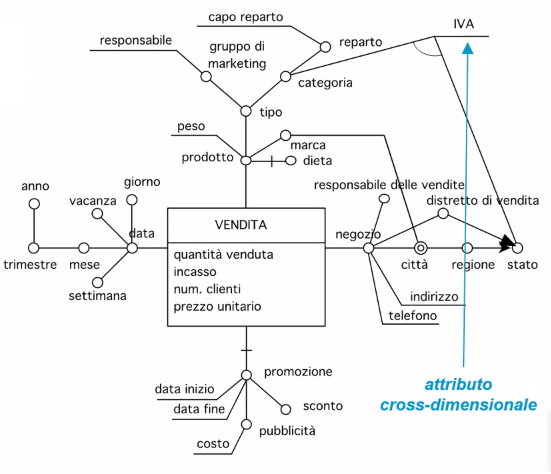
\includegraphics[width=0.7\linewidth]{img/crossdiv.png}
		\caption{Costrutti:Convergenza e Attributo cross-dimensionale}
	\end{center}
\end{figure}
\subsubsection{Arco multiplo}
\begin{info}[Quante volte compare questo costrutto?]
	Molto raro, perché ha implicazioni molto pesanti.
\end{info}
Modella un'associazione molti a molti tra due attributi dimensionali. Dal punto di vista grafico si aggiunge un arco.\newline
Apparentemente sembra non avere grossi impatti, e invece ce ne sono eccome.\newline
Ragioniamo sul seguente DFM:
\begin{figure}[H]
	\begin{center}
		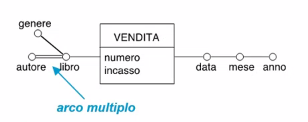
\includegraphics[width=0.55\linewidth]{img/mult.PNG}
		\caption{Costrutto: Arco Multiplo}
	\end{center}
\end{figure}
\noindent Esistono alcuni libri che hanno più autori, ecco una tabella di esempio:
\begin{figure}[H]
	\begin{center}
		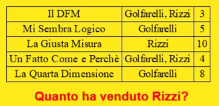
\includegraphics[width=0.4\linewidth]{img/rizzi-golfarelli.PNG}
		\caption{Vendite di Rizzi e Golfarelli}
	\end{center}
\end{figure}
\noindent\textit{"Quanto hanno venduto Rizzi e Golfarelli?}\newline\newline
Golfarelli: \textbf{20}\newline
Rizzi: \textbf{17}\newline
Totale: \textbf{37}\newline\newline
Corretto? No, perché abbiamo fatto \textbf{double counting}, ovvero abbiamo conteggiato più volte gli stessi elementi.\newline
I valori di Rizzi e Goldarelli però sono giusti, solo il totale è sbagliato.
Ci sono diversi modi per fronteggiare questa situazione.
\begin{itemize}
	\item Togliere l'autore, ma l'autore ai fini analitici è un concetto chiave, quindi non possiamo rimuoverlo.
	\item Effettuare una pesatura, per esempio in questo caso la vendita di un libro che ha due autori attribuisce 0.5 vendite a ciascuno. In questo caso i calcoli si trasformano:\newline\newline
	Golfarelli: \textbf{16.5}\newline
	Rizzi: \textbf{13.5}\newline
	Totale: \textbf{30}\newline\newline
	La proprietà che abbiamo utilizzato si chiama \textit{summarizability}, attraverso cui è possibile calcolare il totale a partire da dei parziali. L'arco multiplo viola questa proprietà. Effettuare una somma pesata ripristina questa proprietà.
\end{itemize}
\noindent Come possiamo trasformare un arco multiplo per non avere questi problemi?
\begin{figure}[H]
	\begin{center}
		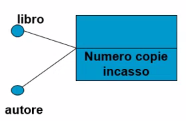
\includegraphics[width=0.4\linewidth]{img/removemult.PNG}
		\caption{Rimozione Arco Multiplo}
	\end{center}
\end{figure}
\noindent Attaccando l'attributo dimensionale autore al fatto e non al libro l'associazione resta molti a molti, apparentemente abbiamo raggiunto il nostro obiettivo. L'effetto collaterale in questo caso si sposta però sulle istanze.
\begin{itemize}
	\item La cardinalità degli eventi primari aumenta, infatti ora le celle del cubo sono di più, perché per esempio per la prima vendita (Il DFM, di Golfarelli e Rizzi) non avrò più una cella sola, ma due. I due eventi primari in questo caso solo la vendita effetuata da Golfarelli e la vendita effettuata da Rizzi. Il problema si ripercuote sugli eventi.\newline
	Che valori finirebbero infatti in numero ed incasso? Se scriviamo "3" in numero non ci liberiamo comunque del double counting, scrivendo 1.5 stiamo forzando la pesatura dentro il cubo.\newline
	\item Secondario: Un libro potrebbe essere associato ad autori sbagliati. Architetturalmente è sbagliato, ma l'ETL aiuta ad evitarlo.
\end{itemize}
\noindent\textbf{Morale}: La soluzione in blu è tecnicamente possibile, ma molto problematica.
Scopriremo più avanti (nella progettazione logica) che avremo strumenti molto flessibili per permetterci di effettuare pesature attraverso la trasformazione subita dall'arco multiplo. Quindi la soluzione con arco multiplo è da preferire alla prima.
\subsubsection{Gerarchia Incompleta}
\begin{info}[Quante volte compare questo costrutto?]
	Negli esercizi quasi mai, nella realtà abbastanza spesso.
\end{info}
Si tratta di una gerarchia in cui, per alcune istanze, risultano assenti in quanto non noti o non definiti, uno o più livelli di aggregazione.\newline
Capita spesso di vedere questo tipo di costrutto nelle reali gerarchie geografiche. per esempio a San Marino non esiste il concetto di regione o di provincia, ma solo di comuni, mentre in Città del Vaticano non esiste nemmeno un comune.
\begin{figure}[H]
	\begin{center}
		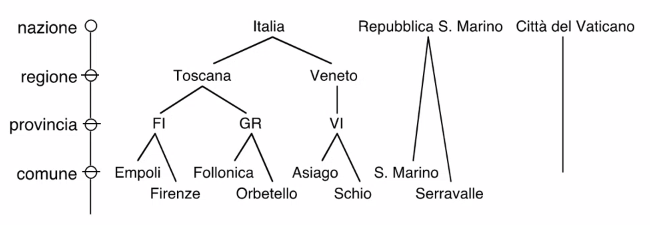
\includegraphics[width=0.9\linewidth]{img/incoml.PNG}
		\caption{Costrutto: Gerarchia Incompleta}
	\end{center}
\end{figure}
\noindent costrutto non è da confondere con l'arco opzionale, che taglia via completamente l'albero (tutto o niente). In questo caso il costrutto è più fine. In questo caso particolare l'unica cosa certa è che la nazione esiste sempre.
\subsubsection{Gerarchia Ricorsiva}
\begin{info}[Quante volte compare questo costrutto?]
	Rarissimo, si usa solo quando strettamente necessario perché portano a problemi di prestazioni.
\end{info}
Si tratta dell'ultimo costrutto in grado di creare un ciclo. In tutti gli altri casi il ciclo è non direzionato, in questo caso lo è.\newline
Il problema in questo caso è che essendo ricorsiva non possiamo sapere quanti livelli ci sono.\newline
Le relazioni padre-figlio tra i livelli sono consistenti, ma le istanze possono avere lunghezze differenti.\newline
Sembra che però il livello gerarchico creato sia molto simile a quello che avevamo nel caso della gerarchia incompleta. Sicuramente esiste qualcosa in comune, entrambe le gerarchie hanno un numero variabile di livelli, ma:
\begin{itemize}
	\item Nella gerarchia incompleta il numero massimo di livelli è fisso. In quella ricorsiva no.
	\item Nella gerarchia incompleta ho una semantica di livello, che è assente in quella ricorsiva. Veneto è sicuramente una regione, PU una provincia, esiste un concetto specifico in cui collocare un certo valore. Questo non è vero in quella ricorsiva.La semantica in questo caso è di arco, solo i collegamenti sono mantenuti.
	\item
\end{itemize}
Casi in cui Rizzi ha visto questo tipo di costrutto:
\begin{itemize}
	\item Organigramma, come da esempio in immagine.
	\item Cubi dove è necessario gestire prodotti composti a loro volta da altri prodotti, tutti quanti vendibili.
\end{itemize}
\begin{figure}[H]
	\begin{center}
		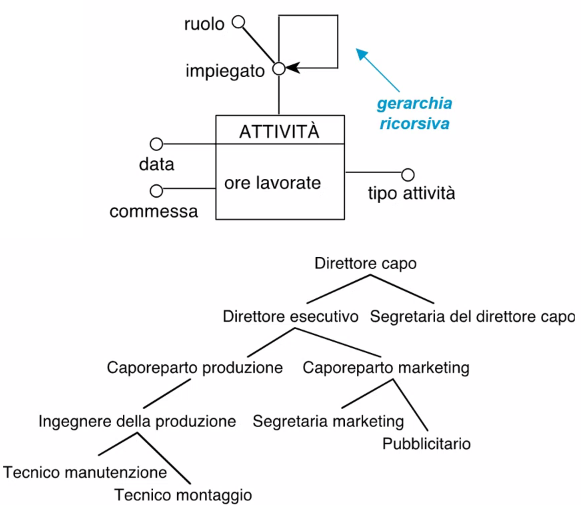
\includegraphics[width=0.6\linewidth]{img/recursive.png}
		\caption{Costrutto: Gerarchia Ricorsiva}
	\end{center}
\end{figure}

\subsubsection{Additività}
\begin{info}[Quante volte compare questo costrutto?]
	SEMPRE, si è sempre tenuti a rappresentarla nei diagrammi.
\end{info}
Esprime in che modo le misure possono essere aggregate in modo corretto.
Ci sono due modi per rappresentare l'additività, quello utilizzato da noi è attraverso una tabella:
\begin{figure}[H]
	\begin{center}
		\includegraphics[width=0.6\linewidth]{img/additività.PNG}
		\caption{Costrutto: Additività}
	\end{center}
\end{figure}
\noindent In ogni incrocio tra misure e gerarchie viene indicato quale o quali indicatori possono essere utilizzati per aggregare.\newline
Per capire come riempire questa matrice dobbiamo avere presenti i tre concetti di misure:
\begin{itemize}
	\item \textbf{Misure di flusso}: Si riferiscono ad un periodo di tempo. Al termine del periodo si assegna un valore quantitativo e cumulativo (ad esempio al termine della giornata quante vendite ho effettuato). Ha sempre senso utilizzare la somma perché le misure sono sempre additive. Ovviamente è anche possibile effettuare altre operazioni, ma ci interessa soprattutto l'additività.\newline
	Queste misure sono additive sempre, anche lungo le gerarchie temporali.
	\begin{info}[Esempio:]
		\newline Se oggi nel negozio sotto casa ho venduto 5 lattine di Coca-Cola e 3 lattine di Fanta posso dire di aver venduto 8 lattine? \textbf{Ovviamente sì}\newline
		Aggreghiamo su negozio... Se ho due negozi e in uno ho venduto 3 PC e nell'altro 9, posso dire di aver venduto 12 PC? \textbf{Ovviamente sì}\newline
		Aggreghiamo temporalmente... Se ho venduto ieri 3 dolci e oggi 6, posso dire di aver venduto complessivamente 9 dolci? \textbf{Ovviamente sì}\newline
	\end{info}
	\item \textbf{Misure di livello}: La valutazione avviene in un particolare istante temporale (quanti prodotti ho nel magazzino in questo momento?). Queste misure sono additive sempre, tranne lungo le gerarchie temporali.
	\begin{info}[Esempio:]
		\newline Aggregando sule città: se oggi nel magazzino di Cesena ho 3 TV e in quello di Bologna 2 posso dire di avere complessivamente 5 TV? \textbf{Ovviamente sì}\newline
		Aggreghiamo su prodotto... Se ho venduto 3 PC e 5 Smartphone, posso dire di aver venduto 8 prodotti? \textbf{Ovviamente sì}\newline
		Aggreghiamo temporalmente... Se oggi ho 5 TV in magazzino mentre ieri ne avevo 7 (e quindi due sono state vendute), posso dire di averne 13? \textbf{NO}\newline
	\end{info}
	\item \textbf{Misure unitarie}: Sono come le misure di livello, valutate in un preciso istante temporale, ma sono espresse in termine relative (il prezzo di un prodotto, la percentuale di sconto, il cambio valuta etc.). Queste misure non sono mai additive.
	\begin{info}[Esempio:]
		\newline Se nel negozio vicino casa mia la lattina di coca cola costa un euro e in un altro costa 2, posso dire che complessivamente? \textbf{NO}\newline
	\end{info}
	Esistono quindi misure additive e misure non additive. L'additività non è una proprietà della misura, e neanche della gerarchia, è una proprietà che va considerata su entrambi.
	\begin{warn}
		Le misure di base sono tutte considerate additive quando facciamo gli esercizi, se non scriviamo niente dobbiamo considerarle tutte come additive. Solo qualora specifichiamo la non additività dobbiamo specificare quali operatori possiamo applicare.
	\end{warn}
\end{itemize}
